\documentclass[14pt, aspectratio=169, handout]{beamer}
\usetheme{Copenhagen}
\usecolortheme{seahorse}
\setbeamertemplate{navigation symbols}{}
\setbeamertemplate{headline}{}

%\usepackage{pgfpages}
%\pgfpagesuselayout{4 on 1}[a4paper, border shrink=5mm]

\usepackage{graphicx} % Required for inserting images
\usepackage{multicol}
%\usepackage{enumitem}
\usepackage{amsfonts}
\usepackage{amsmath}
\usepackage{xcolor}

%--- commands for transform arrows----------------
\newcommand{\transform}[2]{%
    \begin{tikzpicture}
        % Open circle
        \draw[thick] (0,0) circle (0.1);
        % Line with number above and adjustable length
        \draw[thick] (0.1,0) -- (#2,0) node[midway, above] {#1};
        % Filled circle
        \filldraw[thick] (#2,0) circle (0.1);
    \end{tikzpicture}%
}
\newcommand{\invtransform}[2]{%
    \begin{tikzpicture}
        % filled circle
        \filldraw[thick] (0,0) circle (0.1);
        % Line with number above and adjustable length
        \draw[thick] (0.1,0) -- (#2 -0.1,0) node[midway, above] {#1};
        % open circle
        \draw[thick] (#2,0) circle (0.1);
    \end{tikzpicture}%
}
\newcommand{\verticaltransform}[4]{%
    \begin{tikzpicture}
        % Open circle at the bottom with text below
        \filldraw[thick] (0,0) circle (0.1) node[below=3pt] {$#4$};
        % Vertical line with number on the left
        \draw[thick] (0,0.1) -- (0,#2 -0.1) node[midway, left] {#1};
        % Filled circle at the top with text above
        \draw[thick] (0,#2) circle (0.1) node[above=3pt] {$#3$};
    \end{tikzpicture}%
}
\newcommand{\verticalinvtransform}[4]{%
    \begin{tikzpicture}
        % Open circle at the bottom with text below
        \draw[thick] (0,0) circle (0.1) node[below=3pt] {$#4$};
        % Vertical line with number on the left
        \draw[thick] (0,0.1) -- (0,#2) node[midway, left] {#1};
        % Filled circle at the top with text above
        \filldraw[thick] (0,#2) circle (0.1) node[above=3pt] {$#3$};
    \end{tikzpicture}%
}

\definecolor{darkblue}{RGB}{0, 0, 139}
\definecolor{lightblue}{RGB}{173, 216, 230}

\title{SST1 Übungsstunde 6}
\author{Matteo Dietz}
\date{October 2025}

\begin{document}

\maketitle

\begin{frame}{Themenüberblick}
    \begin{itemize}
        \item \textbf{Analoge Lineare Systeme im Frequenzbereich:}
    \item[] Fouriertransformation: Definition, Eigenschaften und Beispiele
    \item[] Dualität der Fouriertransformation
    \item[] Plancherelsche Identität und Parsevalsche Beziehung
    \end{itemize}
\end{frame}

\begin{frame}{Aufgaben für diese und nächste Woche}
    \begin{itemize}
        \item[] \underline{\textbf{56}}, \underline{\textbf{57}}, 58, \underline{\textbf{59}}, \underline{\textbf{60}}, 61, \underline{\textbf{62}}, 63, \underline{\textbf{64}}, 65, \underline{\textbf{66}}
        \item[] 
        \item[] Die \underline{\textbf{fettgedruckten}} Übungen empfehle ich, weil sie wesentlich zu eurem Verständnis der Theorie beitragen und/oder sehr prüfungsrelevant sind.
    \end{itemize}
\end{frame}

\begin{frame}{Analoge Lineare Systeme im Frequenzbereich}
\begin{itemize}
    \item \textbf{Motivation}
\end{itemize}
\begin{center}
     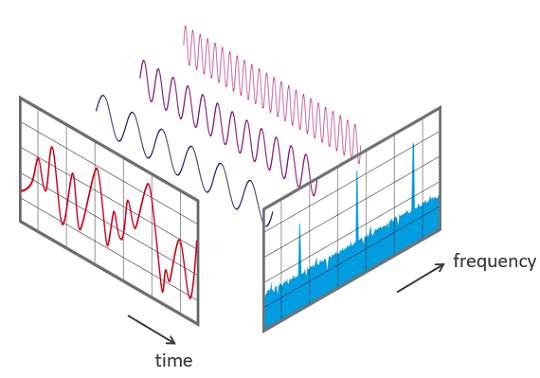
\includegraphics[width=0.65\linewidth]{figures/Zeit_und_Frequenzbereich.png}
\end{center} 
\end{frame}

\begin{frame}{Fouriertransformation}
    \begin{itemize}
    \item \textbf{Fouriertransformation (FT)}:
    \item[] \fcolorbox{darkblue}{lightblue}{%
\parbox{\dimexpr\linewidth-2\fboxsep-2\fboxrule\relax}{
    $$\hat{x}(f) = (\mathcal{F}x)(f) = \int_{-\infty}^{\infty}x(t)e^{-2\pi i f t}\text{d}t$$
}}%
    \item[] 
    \item[] 
    \item \textbf{Inverse Fouriertransformation (IFT)}:
    \item[] \fcolorbox{darkblue}{lightblue}{%
\parbox{\dimexpr\linewidth-2\fboxsep-2\fboxrule\relax}{
    $$x(t) = (\mathcal{F}^{-1}\hat{x})(t) = \int_{-\infty}^{\infty}\hat{x}(f)e^{2\pi i f t}\text{d}f$$
}}%
\end{itemize}
\end{frame}

\begin{frame}{Fouriertransformation: Hinweise}
    \begin{itemize}
        \item KomA/NuS 2: FT und IFT waren definiert als:
$$\hat{x}(\omega) = \int_{-\infty}^{\infty} x(t) e^{-i\omega t}\text{d}t, \hspace{20pt} x(t)=\frac{1}{2\pi} \int_{-\infty}^{\infty} \hat{x}(\omega)e^{i\omega t} \text{d}\omega$$
    \item In SST1 haben wir $t$ und $f$ als Parameter  anstatt $t$ und $\omega$
    \item[] 
    \item $\omega = 2\pi f \implies \text{d}\omega = 2\pi \text{d}f \implies$ kein Vorfaktor $1/(2\pi)$ in IFT
    \end{itemize}
\end{frame}

\begin{frame}{Fouriertransformation: Hinweise}
    \begin{itemize}
        \item Die Fouriertransformation ist eine \textbf{lineare Abbildung}. (\textbf{Additivität} \& \textbf{Homogenität})
        \item[] 
        \item \alert{Berechnet die FT und IFT mithilfe der Transformationstabellen.}
        \item[] 
        \item An der Prüfung muss man eigentlich nie die Integrale der FT berechnen. Es gibt immer einen Kunstgriff, nachdem man die FT von der Tabelle ablesen kann.
    \end{itemize}
\end{frame}

\begin{frame}{Riemann-Lebesgue Lemma}
    \begin{itemize}
        \item Es sei $x$ ein absolut integrierbares Signal, d.h. $x \in L^1$.
        \item[] 
        \item[]  Dann ist $(\mathcal{F}x)(f) = \hat{x}(f)$ stetig und $\displaystyle\lim_{|f| \to \infty} \hat{x}(f) = 0$.
    \end{itemize}
\end{frame}

\begin{frame}{Verschiebung im Zeitbereich}
    
\end{frame}

\begin{frame}{Faltung im Zeitbereich}
    
\end{frame}

\begin{frame}{Aufgaben}
    \begin{itemize}
        \item \textbf{Aufgabe 58.b)}
        \item[] 
        \item \textbf{Aufgabe 60.b)}
        \item[] 
        \item \textbf{Aufgabe 64.b)}
    \end{itemize}
\end{frame}

\begin{frame}{Dualität der Fouriertransformation}
    \includegraphics[width=0.45\linewidth]{figures/dualität_1.png}
    \includegraphics[width=0.45\linewidth]{figures/dualität_2.png}
\end{frame}

\begin{frame}{Beispiel}
    
\end{frame}

\begin{frame}{Parseval und Plancherel}
    \fcolorbox{darkblue}{lightblue}{%
    \parbox{\dimexpr\linewidth-2\fboxsep-2\fboxrule\relax}{
    \begin{center}
        \textbf{Plancherelsche Identität:}
    \end{center}
    $$\langle x, y \rangle = \int_{-\infty}^{\infty} x(t)y^\ast (t)\text{d}t = \int_{-\infty}^{\infty}\hat{x}(f)\hat{y}(f)\text{d}f = \langle \hat{x}, \hat{y} \rangle$$
    \begin{center}
        \textbf{Parsevalsche Beziehung:}
    \end{center}
    $$||x||^2 = \langle x, x \rangle = \int_{-\infty}^{\infty} |x(t)|^2\text{d}t = \int_{-\infty}^{\infty}|\hat{x}(f)|^2\text{d}f = \langle \hat{x}, \hat{x} \rangle = ||\hat{x}||^2$$
    }}
\end{frame}

\begin{frame}{Plancherelsche Identität}
    \begin{itemize}
    \item \textbf{Theorem}: Wenn $f,g \in L^2(\mathbb{R})$, dann gilt $\langle x, y\rangle = \langle \hat{x}, \hat{y}\rangle$
    \item[] $\implies \mathcal{F}$ ist längenerhaltend und winkelerhaltend
    \item \textbf{Beweis}:
    \item[]
    \item[]
    \item[]
    \item[]
    \item[]
    \item[]
    \item[]
\end{itemize}
\end{frame}

\begin{frame}{Aufgaben}
    \begin{itemize}
        \item \textbf{Aufgabe 66}
        \item[]
        \item \textbf{Prüfungsaufgabe: Sommer 2020, Aufgabe 4.a)}
        \item[]
        \item \textbf{Prüfungsaufgabe: Sommer 2019, Aufgabe 2}
    \end{itemize}
\end{frame}

\end{document}
